\section{Instruction set}
L'AVR esegue 1 istruzione per clock, non è propriamente così in quanto alcune istruzioni hanno necessità di più cicli di clock e tutte le istruzioni vogliono un clock per il fetch ed almeno uno per l'esecuzione.
E' vero però che sfruttando la pipeline a 2 livelli che la CPU ci mette a disposizione riusciamo ad eseguire 2 istruzioni in 2 cicli di clock, quindi in media abbiamo 1 istruzione per clock.

\subsection{Istruzioni aritmetiche}

\subsubsection{ADIW}
Somma un operando immediato a 16 bit ad una coppia di registri consecutivi:
\begin{verbatim}
    ADIW r10, 0x1010
        # Somma 0x1010 alla coppia di registri r11:r10
\end{verbatim}

\subsubsection{SBIW}
Sottrae un operando immedato a 16 bit ad una coppia di registri consecutivi:
\begin{verbatim}
    SBIW r10, 0x101
        # Sottrae 0x1010 alla coppia di registri r11:r10
\end{verbatim}

\subsubsection{MUL}
Esegue una moltiplicazione:
\begin{verbatim}
    MUL rx, ry
        # Esegue il prodotto tra i registri specificati
        # e pone il risultato in r1:r0
        # r1:r0 non possono essere usati per porci
        # i fattori
\end{verbatim}

NB: esistono diverse moltiplicazioni per i 3 casi possibili, in più quelli per i numeri in virgola fissa:
\begin{itemize}
    \item MUL: moltiplicazione tra numeri senza segno
    \item MULS: moltiplicazione tra numeri con segno
    \item MULSU: moltiplicazione tra un numeo signed ed uno unsigned
    
    \item MULF: moltiplicazione tra numeri in virgola fissa
\end{itemize}


\subsection{Istruzioni di salto}
\subsubsection{RJMP}
Quando il processore sta eseguendo le istruzioni mantiene l'indirizzo della prossima istruzione da eseguire nel registro Program Counter (PC), modificando questo registro possiamo eseguire dei salti.
L'istruzione RJMP prende come operando un numero, con segno, che indica quanto dobbiamo aggiungere al PC corrente per andare all'istruzione alla quale vogliamo saltare.
Nella pratica questa istruzione produce:
\begin{verbatim}
    PC <- PC + 1 + k
\end{verbatim}
l'aggiunta di 1 viene fatta alla fine della fase di fetch, successivamente si somma il $k$ specificato come operando.

\subsubsection{IJMP}
Salta all'indirizzo contenuto nel registro $Z$.
Compie un salto indiretto assoluto in quanto si deve specificare tutto l'indirizzo in $Z$ e non solo l'offset da sommare.

NB: i salti incondizionati ci mettono sempre 2 cicli interi in quanto il meccanismo di prefetch non può funzionare, va quindi invalidata la pipeline che porta a perdere un ciclo.

\subsubsection{JMP}
Salta all'indirizzo specificato come operando.
Questa istruzione ci mette 3 cicli di clock in quanto l'operando è a 16 bit ed in più deve sempre invalidare la pipeline.

\subsubsection{CPSE}
L'istruzione esegue una comparazione, dopodiché skippa l'istruzione seguente se gli operandi sono uguali.
\begin{verbatim}
    CPSE r0, r1
    JMP not_equal
    JMP equal
        # se r0 == r1 skippa il salto a not_equal
        # ed esegue quello a equal
\end{verbatim}

NB: la durata di questa istruzione dipende se skippa (invalidare la pipeline) o non skippa.

\subsubsection{BREQ - BRNE}
\begin{itemize}
    \item BREQ esegue il salto relativo se Zero flag = 1
    \item BREQ esegue il salto relativo se Zero flag = 0
\end{itemize}

Queste istruzioni di salto condizionato di solito sono precedute da una CP, quindi si riferiscono a quella comparazione.

\subsubsection{BRCS - BRCC}
\begin{itemize}
    \item BRCS esegue il salto relativo se Carry flag = 1
    \item BRCC esegue il salto relativo se Carry flag = 0
\end{itemize}

\subsubsection{BRSH - BRLO}
\begin{itemize}
    \item BRSH: alias per BRCC, salta se maggiore o uguale
    \item BRLO: alias per BRCS, salta se minore
\end{itemize}
Si usano per i numeri naturali.

\subsubsection{BRGE - BRLT}
\begin{itemize}
    \item BRGE: salta se maggiore o uguale
    \item BRLT: salta se minore
\end{itemize}
Si usano per numeri interi.


\subsection{Istruzioni per dialogare con le periferiche}
Abbiamo già visto come le periferiche siano inserite nello spazio di memoria tra gli indirizzi 0x0020 e 0x005F, possiamo dunque leggere e scrivere usando le istruzioni che abbiamo già visto come LDS - STS.
Tuttavia dato che la comunicazione con le periferiche è frequente esistono delle istruzioni un po' più specifiche: IN per leggere da una periferica e OUT per scrivere su una periferica.

Queste istruzioni prevedono l'utilizzo di un \emph{peripheral address} ottenuto semplicemente come: indirizzo reale - 0x0020.

Queste istruzioni sono inoltre più veloci dato che l'indirizzo è a 8 bit e possono accedere esclusivamente ad indirizzi nello spazio delle periferiche!

\begin{verbatim}
    LDS r9, 0x0020
    IN r9, 0x00
        # fanno la stessa cosa
        
    STS 0x0020, r9
    OUT 0x00, r9
        # fanno la stessa cosa
\end{verbatim}

\subsection{Operazioni sui bit}
\begin{itemize}
    \item SBI P, b: setta il b-esimo bit del registro P di I/O
    
    \item CBI P, b: pulisce il b-esimo bit del registro P di I/O
\end{itemize}

\subsubsection{Shift e rotazione}
\begin{itemize}
    \item LSL: shifta tutti i bit di un registro a sinistra, inseriscono il MSB nel CF ed uno 0 come LSB
    \begin{figure}[H]
        \centering
        
\includegraphics[width=250px]{images/6_Instruction_set/LSL.png}
    \end{figure}
    
    \item LSR: shifta tutti i bit di un registro a destra, inseriscono il LSB nel CF ed uno 0 come MSB
    \begin{figure}[H]
        \centering
        
\includegraphics[width=250px]{images/6_Instruction_set/LSR.png}
    \end{figure}
\end{itemize}
Lo shift logico si usa per moltiplicare per 2 (a sinistra) o dividere per 2 (a destra).
Se il numero è con segno e lo moltiplico per due potrebbe non essere rapprsentabile, in tal caso il CF viene settato ad 1.

Nella divisione invece con segno il risultato dovrebbe essere sempre rappresentabile, tuttavia se inserisce lo 0 in testa questo non è più vero:

$$ -1: 11111111 \xrightarrow{} 011111111 : +127 $$
Per risolvere dovrei far entrare come bit più significativo una copia dello stesso MSB, esiste pertanto l' istruzione ASR:
\begin{figure}[H]
    \centering
    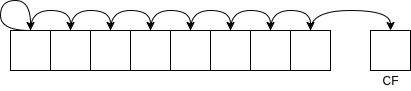
\includegraphics[width=250px]{images/6_Instruction_set/ASR.png}
\end{figure}
Ricopiare il MSB è detto \emph{estensione del segno}.
Questa operazione va fatta anche quando si vuole portare un numero con segno da 8 a 16 bit.

Si noti che dividere -1 con lo shift aritmetico a destra produce ancora -1.
Per definizione la divisione è:
$$ \frac{p}{q} \text{ tc } nq + r = p $$
con $n,r$ unici.

Es: 
$$ \frac{11}{3} \xrightarrow{} 3 \cdot 3 + 2 = 11 $$
$$ 4 \cdot 3 - 1 = 11 $$
$$ 2 \cdot 3 + 5 = 11 $$
per risolvere l'ambiguità si impone $ 0 \leq r \leq q-1 $, se p è negativo il resto deve sempre essere positivo, quindi sempre nell'esempio può valere solo 0, 1, 2.
Si ha quindi quoziente -4 e resto 1.

Es:
$$ -\frac{70}{8} \xrightarrow{} n=-8, r=-6 $$
Sommo 8 al resto e sottraggo 1 al quoziente:
$$ n=-9, r=2 $$

\subsection{Struttura degli opcode}
Il file instruction\_set.pdf contiene delle spiegazioni maggiori sul set di istruzioni dell' AVR. Si nota un certo pattern tra gli opcode:
\begin{itemize}
    \item BREQ, BRCS hanno lo stesso opcode ma cambiano gli ultimi 3 bit, quei bit sono utilizzati per indicare quale dei flag di SREG è di interesse:

    Es: $000 \xrightarrow{}$ carry flag,
    $001 \xrightarrow{}$ zero flag

    \begin{figure}[H]
        \centering
        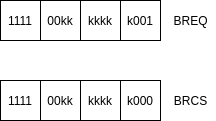
\includegraphics[width=150px]{images/6_Instruction_set/BREQ_BRCS_opcode.png}
    \end{figure}
    
    \item BRCC in confronto a BRCS ha opcode diverso (i primi 13 bit) ma gli ultimi 3 bit identici, appunto perché controllano lo stesso flag
    
    \begin{figure}[H]
        \centering
        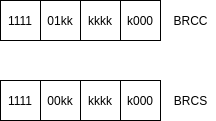
\includegraphics[width=150px]{images/6_Instruction_set/BRCC_BRCS_opcode.png}
    \end{figure}
    
    \item LDI ha 4 bit per indirizzare il registro destinatario, si assume il MSB come 1 quindi possiamo indirizzare i registri da 16 a 31, questo vale per tutte le istruzioni con operando immediato

    \begin{figure}[H]
        \centering
        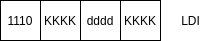
\includegraphics[width=150px]{images/6_Instruction_set/LDI_opcode.png}
    \end{figure}

\end{itemize}

Questo processore è a 8 bit tuttavia le istruzioni sono codificate su 16 bit.
Questo ci permette di avere molte più istruzioni normali e meno istruzioni che sforano andando sui 32 bit (alcuni esempi sono la CALL e la JMP che vogliono l'indirizzo per intero nell' istruzione).
Questa caratteristica porta ad avere una notevole \emph{code density} quindi nello stesso spazio ci sono molte più istruzioni che se fossero codificate su 32 bit.





